\documentclass[fleqn]{article}
\oddsidemargin 0.0in
\textwidth 6.0in
\thispagestyle{empty}
\usepackage{import}
\usepackage{amsmath}
\usepackage{graphicx}
\usepackage{flexisym}
\usepackage{calligra}
\usepackage{amssymb}
\usepackage{bigints} 
\usepackage[english]{babel}
\usepackage[utf8x]{inputenc}
\usepackage{float}
\usepackage[colorinlistoftodos]{todonotes}


\DeclareMathAlphabet{\mathcalligra}{T1}{calligra}{m}{n}
\DeclareFontShape{T1}{calligra}{m}{n}{<->s*[2.2]callig15}{}
\newcommand{\scriptr}{\mathcalligra{r}\,}
\newcommand{\boldscriptr}{\pmb{\mathcalligra{r}}\,}

\definecolor{hwColor}{HTML}{AD53BA}

\begin{document}

  \begin{titlepage}

    \newcommand{\HRule}{\rule{\linewidth}{0.5mm}}

    \center

    \begin{center}
      
\includegraphics[height=11cm, width=11cm]{asu.png}
    \end{center}

    \vline

    \textsc{\LARGE Classical Parts/Field/Matter II}\\[1.5cm]

    \HRule \\[0.5cm]
    { \huge \bfseries Problem Set Four}\\[0.4cm] 
    \HRule \\[1.0cm]

    \textbf{Behnam Amiri}

    \bigbreak

    \textbf{Prof: Maulik Parikh}

    \bigbreak

    \textbf{{\large \today}\\[2cm]}

    \vfill

  \end{titlepage}

  \begin{enumerate}
    \item Some people are afraid of living near power lines.  A $50 ~ kV$ direct current power line consists of two wire conductors 2 m apart. If the
    power line is transmitting $10 MW$ of power, what is the strength of the
    magnetic field halfway between the conductors?

      \textcolor{hwColor}{
        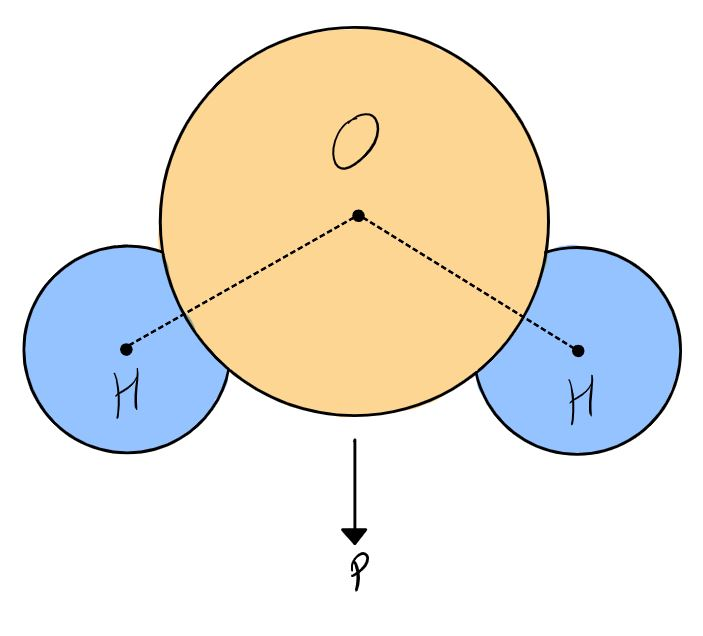
\includegraphics[height=6cm, width=9cm]{1.JPG}
        \\
        We learned in the past that $P=V \times I$ so we have:
        \\
        \\
        $
          P=V \times I=\dfrac{P}{V}=\dfrac{10 MW}{50 ~ kV}=\dfrac{10 \times 10^6 ~ W}{50 \times 10^3 ~ V}
          \\
          \\
          \\
          \therefore ~~~ I=200 ~ A ~~~~ \checkmark
        $
        \\
        \\
        We just found the current in the wires. On page 233 we have the Ampère's law as:
        \\
        \\
        $
          \bigoint B.d\ell=\mu_0 ~ I_{enc}
        $
        \\
        \\
        On page 234 we got that $B=\dfrac{\mu_0 I}{2 \pi R}$ which is the magnetic field a distance $R$ from a 
        long straight wire carrying a steady current. Whatever plane we assume these magnetic fields are on the 
        net magnetic field is normal to them. Assuming the two magentic fields are on the $x-y$ plane, then 
        $\overrightarrow{B}=\overrightarrow{B_1}+\overrightarrow{B_2}$ is in the $z$ direction.
        \\
        \\
        $
          \overrightarrow{B}=\overrightarrow{B_1}+\overrightarrow{B_2}
          =\dfrac{\mu_0 I}{2 \pi R_1} \hat{z}+\dfrac{\mu_0 I}{2 \pi R_2} \hat{z}
          =\dfrac{\mu_0 I}{2 \pi R} \hat{z}+\dfrac{\mu_0 I}{2 \pi R} \hat{z}
          =\dfrac{\mu_0 I}{\pi R} \hat{z}
          =\dfrac{\mu_0 200}{\pi (1)} \hat{z}
          \\
          \\
          \\
          \therefore ~~~ \overrightarrow{B}=\dfrac{200 ~ \mu_0}{\pi} \hat{z} ~~~ T ~~~~ \checkmark
        $
        \\
        \\
        Note: In order to find the numerical value of $\overrightarrow{B}$ we can simply plug in the value of $\mu_0$ which is 
        $4 \pi \times 10^{-7}$. 
        \\
        \\
      }

    \item \textbf{Animal Magnetism}
    \\
    Andre Geim was awarded the $2000 ~ Ig$ Nobel prize (a parody award given for the most absurd research) for showing that live frogs are
    diamagnetic and can be levitated using a sufficiently strong magnet. Using the formula for the force on a magnetic dipole, 
    $\overrightarrow{F}=\overrightarrow{\nabla} \left(
      \overrightarrow{m}.\overrightarrow{B}
    \right)$,and assuming that the frog has volume $V$ , mass density $\rho$, and is a magnetically linear medium with 
    magnetic susceptibility, $\chi_m \approx 10^{-5}$, calculate the strength of the solenoid magnet in Teslas necessary to
    levitate the frog. Assume that the solenoid is about $L=10 ~ cm$ in
    length and approximate $\overrightarrow{\nabla} B^2 \approx \dfrac{B^2}{L} \hat{z}$. (Geim later redeemed himself
    by winning the 2010 Nobel prize for his work on graphene.)

      \textcolor{hwColor}{
        \\
        This probelm was solved by the help of a paper called \textbf{Of flying frogs and levitrons}.
        We got the following.
        \\
        \\
        $
         \begin{cases}
          \chi_m=0
          \\
          \\
          \overrightarrow{\nabla} B^2 \approx \dfrac{B^2}{L} \hat{z}
          \\
          \\
          \alpha=p \bigints\limits_{0}^{v} dv
          \\
          \\
          \overrightarrow{M}=\overrightarrow{M} V^{-1} ~~~~ \text{Magnetic dipole of the frog}
          \\
          \\
          \overrightarrow{H}=\dfrac{1}{\mu_0} \overrightarrow{B}-\overrightarrow{M} ~~~~~ \overrightarrow{M}=-|\chi_m| \overrightarrow{H}
          \\
          \\
         \end{cases}
         \\
         \\
         \\
         \therefore ~~~ -\chi_m^{-1} \overrightarrow{M}=\dfrac{1}{\mu_0} \overrightarrow{B}-\overrightarrow{M}
         \\
         \\
         \\
         \therefore ~~~ \overrightarrow{M}-\dfrac{\chi_m}{\mu_0} \overrightarrow{B} ~~~~ \text{Since $1-\chi_m \approx 1$}
         \\
         \\
         \\
         \therefore ~~~ \overrightarrow{M}=-\dfrac{\chi_m V}{\mu_0} \overrightarrow{B}
        $
        \\
        \\
        Now we are all set to find the force on magnetic dipole.
        \\
        \\
        $
          \overrightarrow{F}=\left(\overrightarrow{M}.\overrightarrow{\nabla}\right) \overrightarrow{B}
          \\
          \\
          \therefore ~~~ \overrightarrow{F}=\mu \left(\dfrac{1}{2} \nabla |\overrightarrow{B}|^2-\overrightarrow{B} \times \left(\nabla \times \overrightarrow{B}\right)\right)
          \\
          \\
          \\
          \overrightarrow{B} \times \left(\nabla \times \overrightarrow{B}\right)=\overrightarrow{B} \times \overrightarrow{0}
          \\
          \\
          \\
          \therefore ~~~ \overrightarrow{B} \times \left(\nabla \times \overrightarrow{B}\right)=\overrightarrow{0}
          \\
          \\
        $
        Therefore, the force on the magnetic dipole is:
        \\
        \\
        $
          \overrightarrow{F_m}=\dfrac{\mu}{2} \nabla B^2=\dfrac{\mu}{2L} B^2 \hat{z}
          \\
          \\
          \\
          \therefore ~~~ \overrightarrow{F_m}=-\dfrac{\chi_m V}{2 \mu_0 L} B^2 \hat{z} ~~~~ \checkmark
        $
        In order to have the frog to levitate, the gravity and the magnetic force has to be equal but in the opposite directions.
        \\
        \\
        $
          \overrightarrow{F_g}=\overrightarrow{F_m} \Longrightarrow pVg(-\hat{z})=\dfrac{\chi_m V}{2 \mu_0 L} B^2 (-\hat{z})
          \\
          \\
          \\
          \therefore ~~~ |B|=\sqrt{\left(\dfrac{2 \mu_0 Lpg}{\chi_m}\right)} ~~~~ \checkmark
        $
        \\
        \\
        For $\overrightarrow{F_m}$ we have:
        \\
        \\
        $
          \overrightarrow{F_m}=\overrightarrow{\nabla} \left(
            \overrightarrow{m}.\overrightarrow{B}
          \right)=\overrightarrow{\nabla} \left(
            \dfrac{-\chi_m V}{\mu_0}\overrightarrow{B}.\overrightarrow{B}
          \right)=-\dfrac{\chi_m V}{\mu_0} \nabla |B|^2=-\dfrac{k_m V B^2}{L} ~ \hat{z}
          \\
          \\
          \\
          \overrightarrow{F_g}=\overrightarrow{F_m} \Longrightarrow -\dfrac{\chi_m V B^2}{\mu_0 L} \hat{z}=pVg (-\hat{z})
          \\
          \\
          \\
          \therefore ~~~ |B|=\sqrt{\dfrac{L p g \mu_0}{\chi_m}}
          \\
          \\
          \\
          \therefore ~~~ |B|=\sqrt{\dfrac{p \times 0.1 \times 9.8 \times 4 \pi \times 10^{-7}}{10^{-5}}}
          \\
          \\
          \\
          \therefore ~~~ |B|=\dfrac{35}{100} \sqrt{p} ~~~~ T
          \\
          \\
        $
      }

    \pagebreak

    \item \textbf{Hall Effect}
    \\
    The Hall effect was discovered in 1879. It confirms that the charge carriers in electric currents are negatively charged (i.e. are electrons).
    Consider a long conducting slab, infinitely extending in the $\hat{x}$ direction, whose rectangular cross-section has thickness $t$ in 
    the $\hat{y}$ direction and width $w$ in the $\hat{z}$ direction. Let a current $I$ flow in the $+\hat{x}$ direction
    and suppose there is a uniform magnetic field $\overrightarrow{B}=B_0 \hat{y}$. In which direction are the mobile charges deflected if they 
    have positive charge? The deflection leads to an accumulation of charge on the surfaces of the slab (this is the Hall effect), until the 
    corresponding electric field counteracts the magnetic deflection. Find the resulting Hall voltage, in terms of $B_0$, $v$, and the dimensions
    of the slab. Repeat your analysis for negative charge carriers.

      \textcolor{hwColor}{
        \\
        We should start by figuring out what direction the force due to $\overrightarrow{B}$ acts. 
        \\
        \\
        $
          \overrightarrow{F_m}=q  \left(v \times \overrightarrow{B}\right)=q v B \left(\hat{x} \times \hat{y}\right)
          \\
          \\
          \\
          \therefore ~~~ \overrightarrow{F_m}=qvB ~ \hat{z} ~~~~ \checkmark
        $
        \\
        \\
        The Hall effect $\overrightarrow{F_m}-\overrightarrow{F_e}=0$, therfore, we have $qvB_0=qE \Longrightarrow E=vB_0$.
        \\
        \\
        $
          V_{H}=-\bigints\limits_{W}^{0} E ds=Ew=vwB_0
          \\
          \\
          \\
          \overrightarrow{F_m}=-q \left(v \times B\right)=-q (v)(-\hat{x}) \times B_0 \hat{y} \Longrightarrow \overrightarrow{F_m}=qvB \hat{z}
        $
        The reason for the above is that the current tavels in the $\hat{x}$ direction and the negative charges travel in the opposite direction.
        \\
        \\
        $
          |\overrightarrow{F_m}|=|\overrightarrow{F_e}| \Longrightarrow (-q) vB_0=(-q) E \longleftarrow E=vB_0 ~~~~ \checkmark
          \\
          \\
          \therefore ~~~ V_H=-\bigints\limits_{W}^{0} E ds=vB_0 w ~~~~ \checkmark
        $
      }

    \item Two parallel circular loops of wire, each with radius a, have the same axis along the $\hat{z}$ direction. The planes of the loops 
    are located at $z=-\epsilon$ and $z=+\epsilon$, where $\epsilon << a$. Suppose that there is a current $I$ flowing in each of the loops, 
    but in opposite directions, say clockwise (seen from above) in the upper loop, and counter-clockwise in the lower loop. Find the z-value 
    on the axis where the magnetic field is maximal.

      \textcolor{hwColor}{
        \\
        We have two parallel circular loops and there is current $I$ in both of them but in different directions.
        \\
        \\
        $
          \overrightarrow{B}_2(\overrightarrow{r})=\dfrac{\mu_0}{4 \pi} ~ I ~ \bigints \dfrac{d\ell \times \hat{r}}{r^2}
          \\
          \\
          \begin{cases}
            r^2=\left(\epsilon+z\right)^2+a^2
            \\
            \\
            \overrightarrow{B}(\overrightarrow{r})
            \\
            \\
            k=\dfrac{\mu_0}{4 \pi} I
          \end{cases}
          \\
          \\
          \\
          \overrightarrow{B}(\overrightarrow{r})=k \bigints \dfrac{a d\phi \hat{\phi} \times \left(-\dfrac{a \hat{r} +(\epsilon+z) \hat{z}}{r}\right)}{r^2}
          \\
          \\
          \\
          =k \bigints \dfrac{a d\phi \hat{\phi} \times \left(-a \hat{r}+(\epsilon+z) \hat{z}\right)}{r^3}
          =\left[\dfrac{ka^2}{r^3} \bigints\limits_{0}^{2 \pi} d\phi(+\hat{z})\right]
          +\left[\dfrac{ka (\epsilon+z)}{r^3} \bigints\limits_{0}^{2 \pi}\right]
          \\
          \\
          \\
          =\left[\dfrac{ka^2}{r^3} (2\pi) \hat{z}\right]
          +\left[\dfrac{ka(\epsilon+z)}{r^3} \bigints\limits_{0}^{2 \pi} sin(\phi) d\phi \right]
          =\dfrac{2 \pi ~ ka^2}{r^3} \hat{z}
          \\
          \\
          \\
          \therefore ~~~~ \overrightarrow{B}_2(\overrightarrow{r})=\dfrac{\mu_0 a^2}{2 \left[(\epsilon+z)^2+a^2\right]^{3/2}} ~ I ~ \hat{z} ~~~~ \checkmark
          \\
          \\
          \\
          \\
          \\
          \begin{cases}
            r^2=a^2+(-\epsilon+z)^2
            \\
            \\
            \hat{r}=\dfrac{\overrightarrow{r}}{r}
          \end{cases}
          \\
          \\
          \\
          \overrightarrow{B}_1(\overrightarrow{r})=k \bigints \dfrac{d\ell \times \hat{r}}{r^2}
          =k \bigints\limits_{4 \pi}^{7} \dfrac{(-a d\phi \hat{\phi}) \times (-a \hat{r}+(-\epsilon+z) \hat{z})}{r^3}
          \\
          \\
          \\
          =\left[\dfrac{k}{r^3} \bigints (-a d\phi \hat{\phi}) \times (-a \hat{r})\right]
          +\left[\dfrac{k}{r^3} \bigints (-a d\phi \hat{\phi}) \times ((-epsilon+z)\hat{z})\right]
          =k\dfrac{2 \pi a^2}{r^3} (-\hat{z})
          \\
          \\
          \\
          \therefore ~~~ \overrightarrow{B}_1(\overrightarrow{r})=\dfrac{\mu_0 a^2}{2 \left[(-\epsilon+z)^2+a^2\right]^{3/2}} ~ I ~ \hat{-z}
          \\
        $
        \\
        \\
        Since $\overrightarrow{B}=\overrightarrow{B}_1+\overrightarrow{B}_2$ we have:
        \\
        \\
        $
          \therefore ~~~ \overrightarrow{B}=\dfrac{\mu_0 a^2}{2} ~ \left[
            \dfrac{1}{\left[(\epsilon+z)^2+a^2\right]^{3/2}}
            -\dfrac{1}{\left[(-\epsilon+z)^2+a^2\right]^{3/2}}
          \right] I ~ \hat{z} ~~~~ \checkmark
        $
        \\
        \\
        \\
        $
          \dfrac{dB}{dz}=\dfrac{d}{dz} \left[
            \dfrac{\mu_0 I a^2}{2} \left[
              \left((z+\epsilon)+a^2\right)^{3/2}
              -\left((z-\epsilon)^2+a^2\right)
            \right]
          \right] \hat{z} ~~~~ \alpha=\mu_0 I a^2
          \\
          \\
          \\
          \alpha \left[
            \left((z+\epsilon)+a^2\right)^{3/2}
            -\left((z-\epsilon)^2+a^2\right)
          \right]=0
          \\
          \\
          \\
          \therefore ~~~ \dfrac{d}{dz}=\left((z-\epsilon)^2+a^2\right)^{-3/2}
          \\
          \\
          \\
          -\dfrac{3}{2} \left((z+\epsilon)^2+a^2\right)^{-5/2} \dfrac{d}{dz} (z+\epsilon)^2
          \\
          \\
          \\
          \therefore \left(1+\dfrac{\epsilon^2-2z\epsilon}{z^2+a^2}\right)^{5/2} (z+\epsilon)
          =\left(1+\dfrac{\epsilon^2+2z \epsilon}{z^2+a^2}\right)^{5/2} (z-\epsilon)
        $
        \\
        \\
        \\
        Using the Taylor expansion we have:
        \\
        \\
        $
          \begin{cases}
            \left(1+\dfrac{\epsilon^2+2z \epsilon}{z^2+a^2}\right)^{5/2} (z-\epsilon) \approx 1-\dfrac{4z \epsilon}{z^2+a^2}
            \\
            \\
            \left(1+\dfrac{\epsilon^2-2z \epsilon}{z^2+a^2}\right)^{5/2} (z-\epsilon) \approx 1+\dfrac{4z \epsilon}{z^2+a^2}
          \end{cases}
          \\
          \\
          \\
          \left(1-\dfrac{5 z\epsilon}{z^2+a^2}\right) (z+\epsilon)=\left(1+\dfrac{5 z \epsilon}{z^2+a^2}\right) (z-\epsilon)
          \\
          \\
          \\
          \therefore ~~~ 2\epsilon=\dfrac{10 z^2 \epsilon}{z^2+a^2}
          \\
          \\
          \\
          \therefore ~~~ z^2=\pm \dfrac{a^2}{4}
          \\
          \\
          \\
          \therefore ~~~ z=\pm \dfrac{a}{2} ~~~~ \checkmark
          \\
          \\
        $
        What we found is the position of the field at max. 
      }

    \pagebreak

    \item A hollow cone (like an ice cream cone) has vertex angle $2\theta$, slant height $L$ (slant height is measured along the side), 
    and surface charge density $\sigma$. The cone spins around its symmetry axis with angular frequency $\omega$. Find the magnetic field at 
    the tip of the cone.

      \textcolor{hwColor}{
        \\
        See the attached
        \\
      }

    \item Find the vector potential, $\overrightarrow{A}$, for
    \begin{enumerate}
      \item A finite straight wire with current $I$ (flowing in the $+\hat{z}$ direction)
      extending from $z=-z_0$ to $z=+z_0$.

      \textcolor{hwColor}{
        \\
        See the attached
        \\
      }

      \item An infinite straight wire, aligned in the $\hat{z}$ direction, with current
      $I$ flowing in the $+\hat{z}$ direction. (also find $\overrightarrow{B}$ from $\overrightarrow{A}$)

      \textcolor{hwColor}{
        \\
        See the attached
        \\
      }
      
      \item A uniform magnetic field $B_0$ in the $\hat{z}$ direction.

      \textcolor{hwColor}{
        \\
        See the attached
        \\
      }

    \end{enumerate}


    \item A uniform current $I$ flows down a wire of radius $R$ made of a linear material with magnetic susceptibility $\chi_m$. Find the 
    magnetic field as a function of $r$. Also find the bound currents. What is the net bound current flowing down the wire?

      \textcolor{hwColor}{
        \\
        $
          \overrightarrow{B}=\mu ~ \overrightarrow{H}=\mu_0 \left(1+\chi_m\right) \overrightarrow{H}
          \\
          \\
          \\
          I_{enc}=I ~ \dfrac{2 \pi r^2}{2 \pi R^2}=I ~ \dfrac{r^2}{R^2}
          \\
          \\
          \\
          \bigoint H.d\ell=I_{enc} \Longrightarrow |H|=\dfrac{1}{2 \pi r} I_{enc}
        $
        \\
        \\
        $|H|$ is the direction of $\hat{\phi}$ therefore we have the following results:
        \\
        \\
        $
          \overrightarrow{H}=\begin{cases}
            \dfrac{r}{2 \pi R^2} I ~ \hat{\phi} ~~~~~ r<R
            \\
            \\
            \dfrac{1}{2 \pi r} I ~ \hat{\phi} ~~~~~ r\geq R
          \end{cases}
          \\
          \\
          \\
          \\
          \\
          \therefore ~~~ \begin{cases}
            \overrightarrow{B}=\dfrac{\mu_0 r (1+\chi_m)}{2 \pi R^2} I \hat{\phi} ~~~~ r<R
            \\
            \\
            \overrightarrow{B}=\dfrac{\mu_0 (1+\chi_m)}{2 \pi r} I \hat{\phi} ~~~~~ r\geq R
          \end{cases}
        $
        \\
        \\
        Time to calculate the bound currents. We know that $\overrightarrow{M}=\chi_m \overrightarrow{H}$. For the inner side we 
        have:
        \\
        \\
        $
          \overrightarrow{M}=\dfrac{\chi_m r}{2 \pi R^2} I \hat{\phi}
          \\
          \\
          \\
          \overrightarrow{J_B}=\overrightarrow{\nabla} \times \overrightarrow{M}
          =\hat{r} \left(\dfrac{1}{r} \dfrac{\partial ~ M_z}{\partial \phi}-\dfrac{\partial ~ M_{\phi}}{\partial z} \right)
          +\hat{\phi} \left(\dfrac{\partial M_r}{\partial z}-\dfrac{\partial M_z}{\partial r}\right)
          +\hat{z} \dfrac{1}{r} \left(\dfrac{\partial r M_{\phi}}{\partial r}-\dfrac{\partial M_r}{\partial \phi}\right)
          \\
          \\
          \\
          =\dfrac{1}{r} \dfrac{\partial }{\partial r} \left(\dfrac{\chi_m r^2 }{2 \pi R^2}\right) I \hat{z}
          \\
          \\
          \\
          \therefore ~~~ \overrightarrow{J_B}=\dfrac{\chi_m }{\pi R^2} ~ I \hat{z} ~~~~ \checkmark
          \\
          \\
          \\
          \therefore ~~~ \overrightarrow{K_B}=\dfrac{\chi_m}{2 \pi R} ~ I  \hat{\phi} \times \hat{r}
          \\
          \\
          \\
          \therefore ~~~ \overrightarrow{K_B}=\dfrac{\chi_m}{2 \pi R} \left(-\hat{z}\right) ~~~~ \checkmark
        $
        \\
        \\
        \\
        The net bound current flowing down the wire then is:
        \\
        \\
        $
          I_b=\bigints\limits_{0}^{R} \bigints\limits_{0}^{2 \pi} k_b ~ d\phi ~ dr
          +\bigints\limits_{0}^{R} \bigints\limits_{0}^{2 \pi} J_b r ~ d\phi ~ dr
          =\left(\dfrac{\chi_m ~ I}{2 \pi R}\right)\left(2 \pi R\right)\left(-\hat{z}\right)
          +\left(\dfrac{\chi_m ~ I}{\pi R^2}\right)\left(\pi R^2\right)\left(\hat{z}\right)
          \\
          \\
          \\
          \therefore ~~~ I_b=0 ~~~~ \checkmark
        $
        \\
        \\
      }

    \item A wire of circular cross-section with radius $R$ carries a uniformly distributed current, $I$. Suppose the current flows in the $+\hat{z}$ direction.
    Find the magnetic field $\overrightarrow{B}$ at all points inside the wire. Show that a vector potential of the form 
    $\overrightarrow{A}=A_0 \left(x^2+y^2\right) ~ \hat{z}$ will correctly give the
    magnetic field. What is the value of the constant, $A_0$?

      \textcolor{hwColor}{
        \\
        We have the current flows in the $\hat{z}$ direction. By using the right hand rule we can find the direction of the magentic field 
        that can be assumed it is in the direction of $\hat{\phi}$. For this problem we have $I$ as: 
        \\
        \\
        $
          I_{enc}=\dfrac{I \pi r^2}{\pi R^2} \Longrightarrow I_{enc}=\dfrac{r^2}{R^2} ~ I
          \\
          \\
          \\
          \bigoint B.d\ell=\mu_0 ~ I_{enc} \Longrightarrow \bigoint B.d\ell=\mu_0 ~ \dfrac{r^2}{R^2} ~ I
          \\
          \\
          \\
          |B| 2 \pi r=\mu_0 ~ \dfrac{r^2}{R^2} ~ I \Longrightarrow |B|=\dfrac{\mu_0 r}{2 \pi R^2} ~ I ~ \hat{\phi} ~~~~ \checkmark
          \\
          \\
          \\
        $
        In cylindrical coordinate we have $\overrightarrow{A}=A_0 r ~ \hat{z}$.
        \\
        \\
        $
          \overrightarrow{B}= \overrightarrow{\nabla} \times \overrightarrow{A}
          =\hat{r} \left(\dfrac{1}{r} \dfrac{\partial ~ A_z}{\partial \phi}-\dfrac{\partial ~ A_{\phi}}{\partial z} \right)
          +\hat{\phi} \left(\dfrac{\partial A_r}{\partial z}-\dfrac{\partial A_z}{\partial r}\right)
          +\hat{z} \dfrac{1}{r} \left(\dfrac{\partial r A_{\phi}}{\partial r}-\dfrac{\partial A_r}{\partial \phi}\right)
          =-2A_0 ~ r ~ \hat{\phi}
          \\
          \\
          \\
          \therefore ~~~ -2A_0 ~ r ~ \hat{\phi}=\dfrac{\mu_0 r}{2 \pi R^2} I \hat{\phi}
          \\
          \\
          \\
          \therefore ~~~ A_0=-\dfrac{\mu_0}{4 \pi r^2}I ~~~~ \checkmark
        $
        \\
        \\
      }

      \pagebreak

      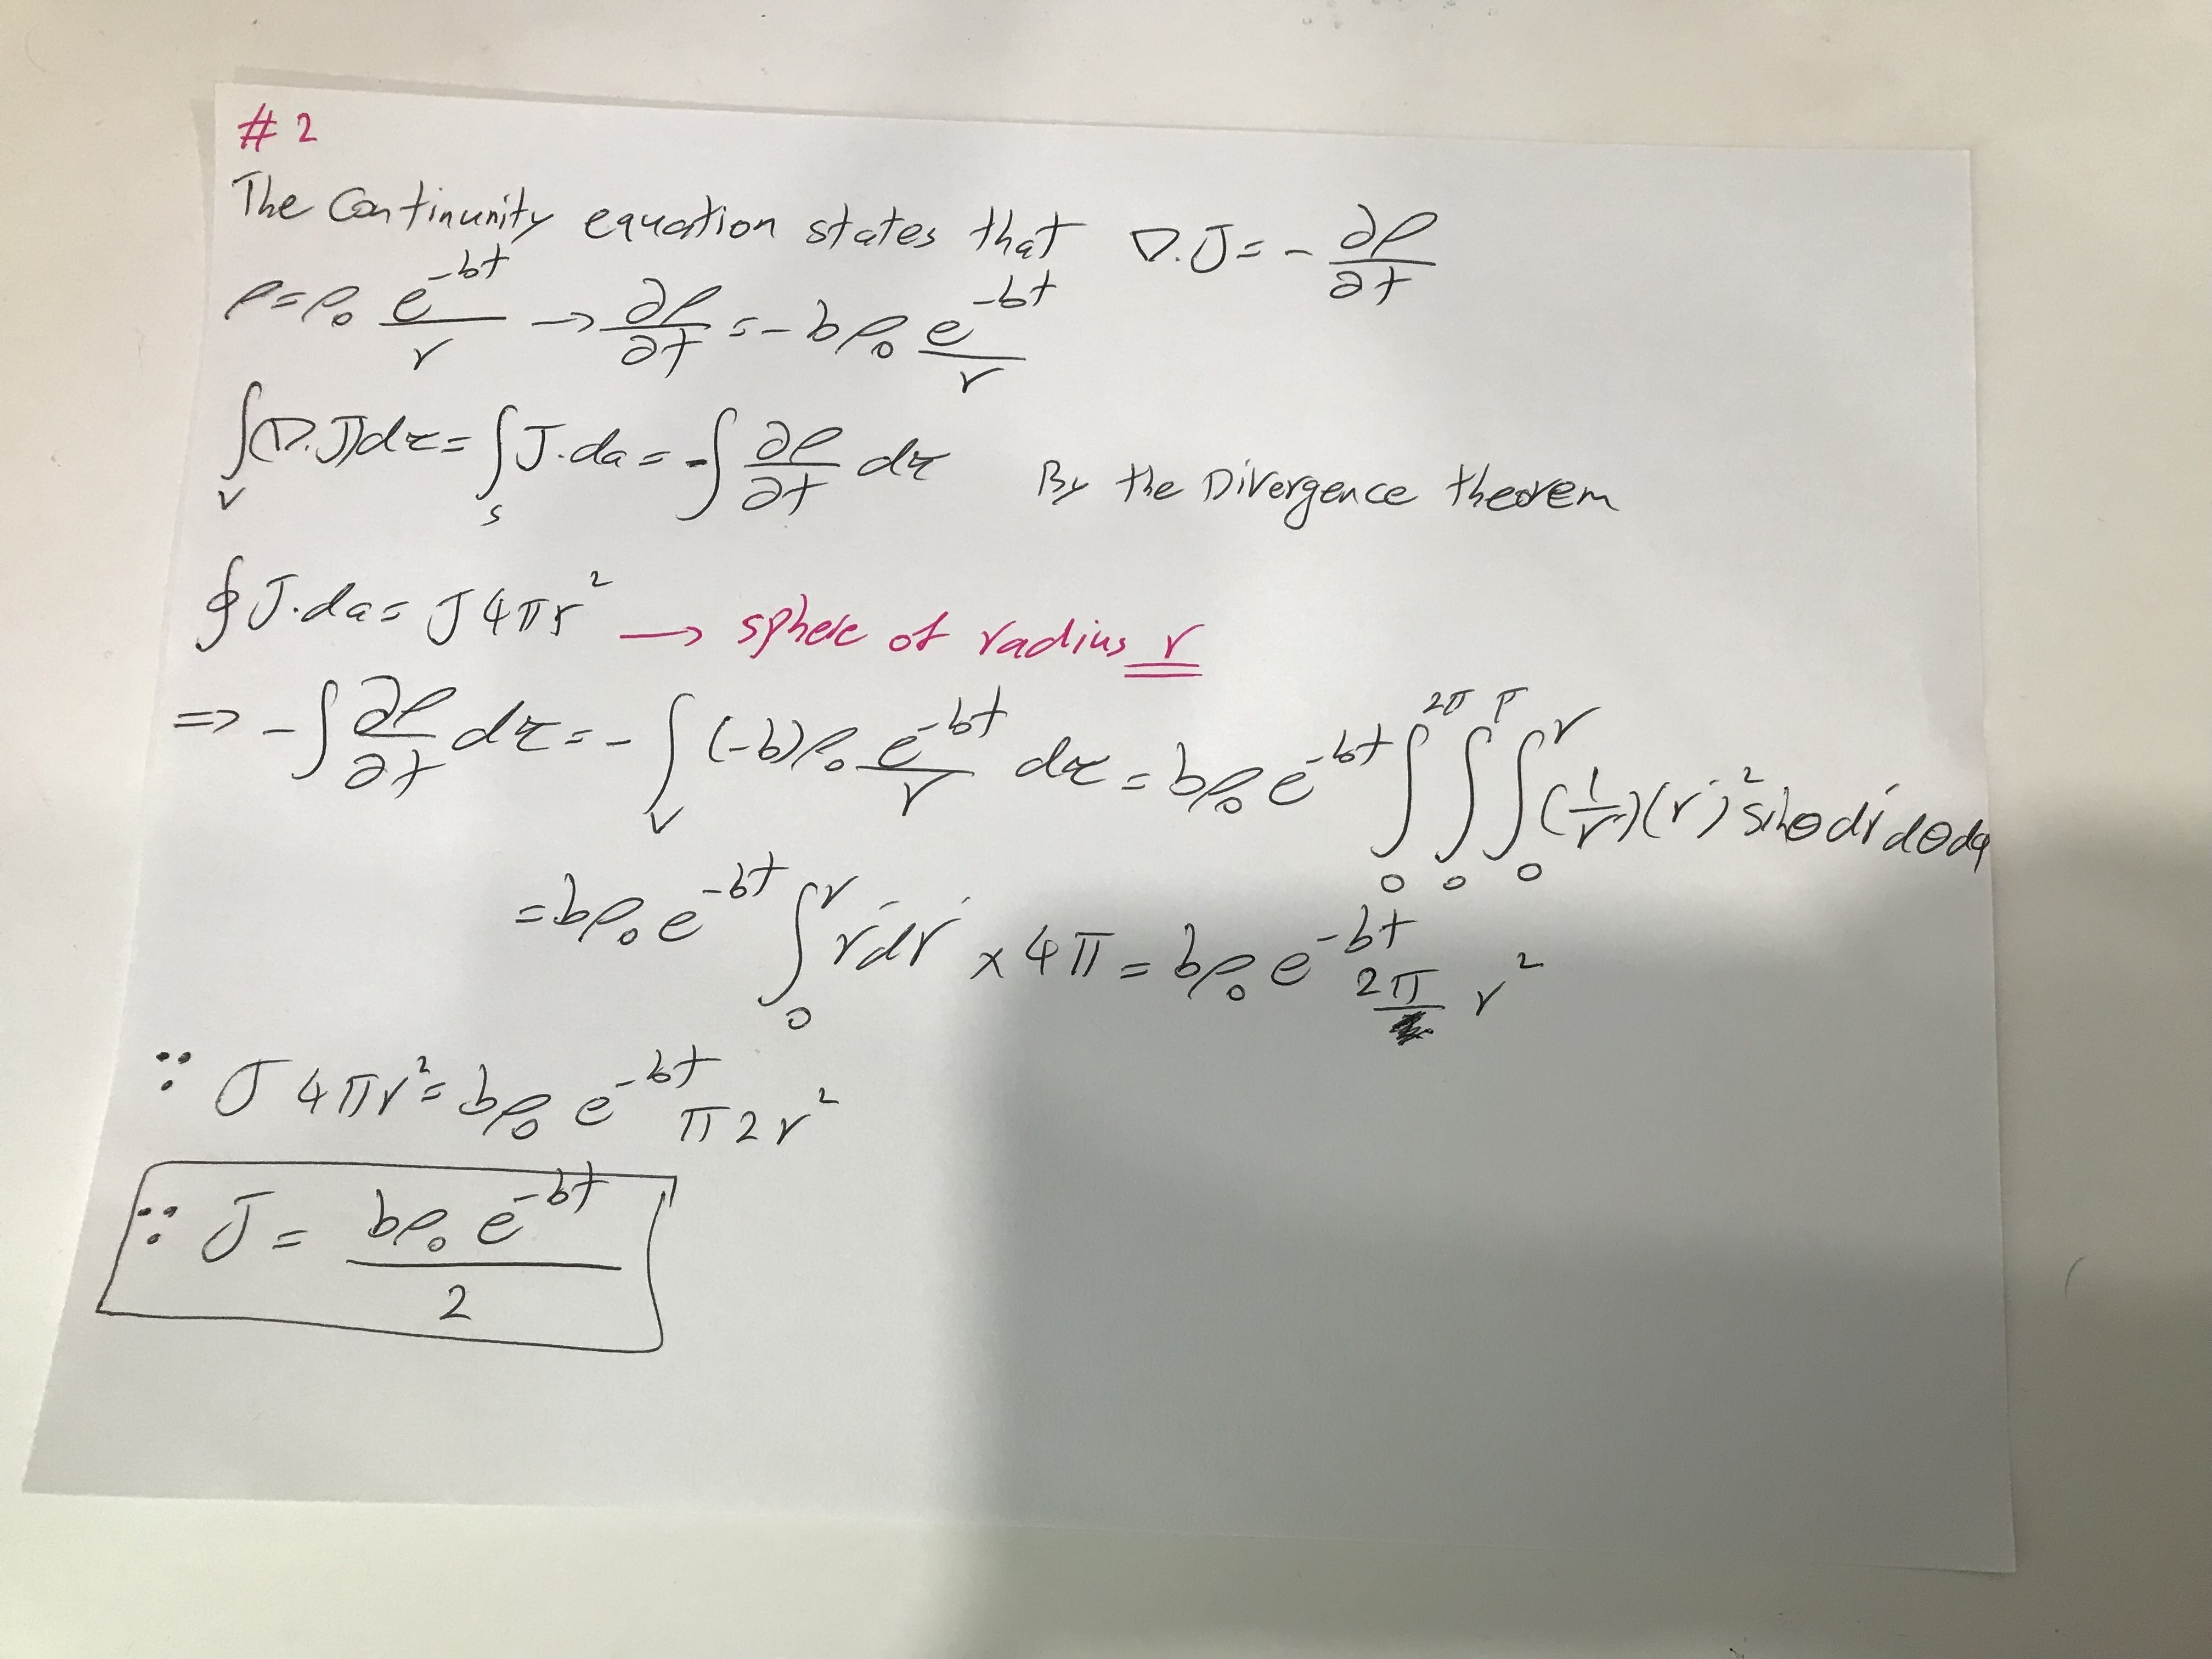
\includegraphics[height=16cm, width=17cm]{2.jpg}

      \pagebreak

      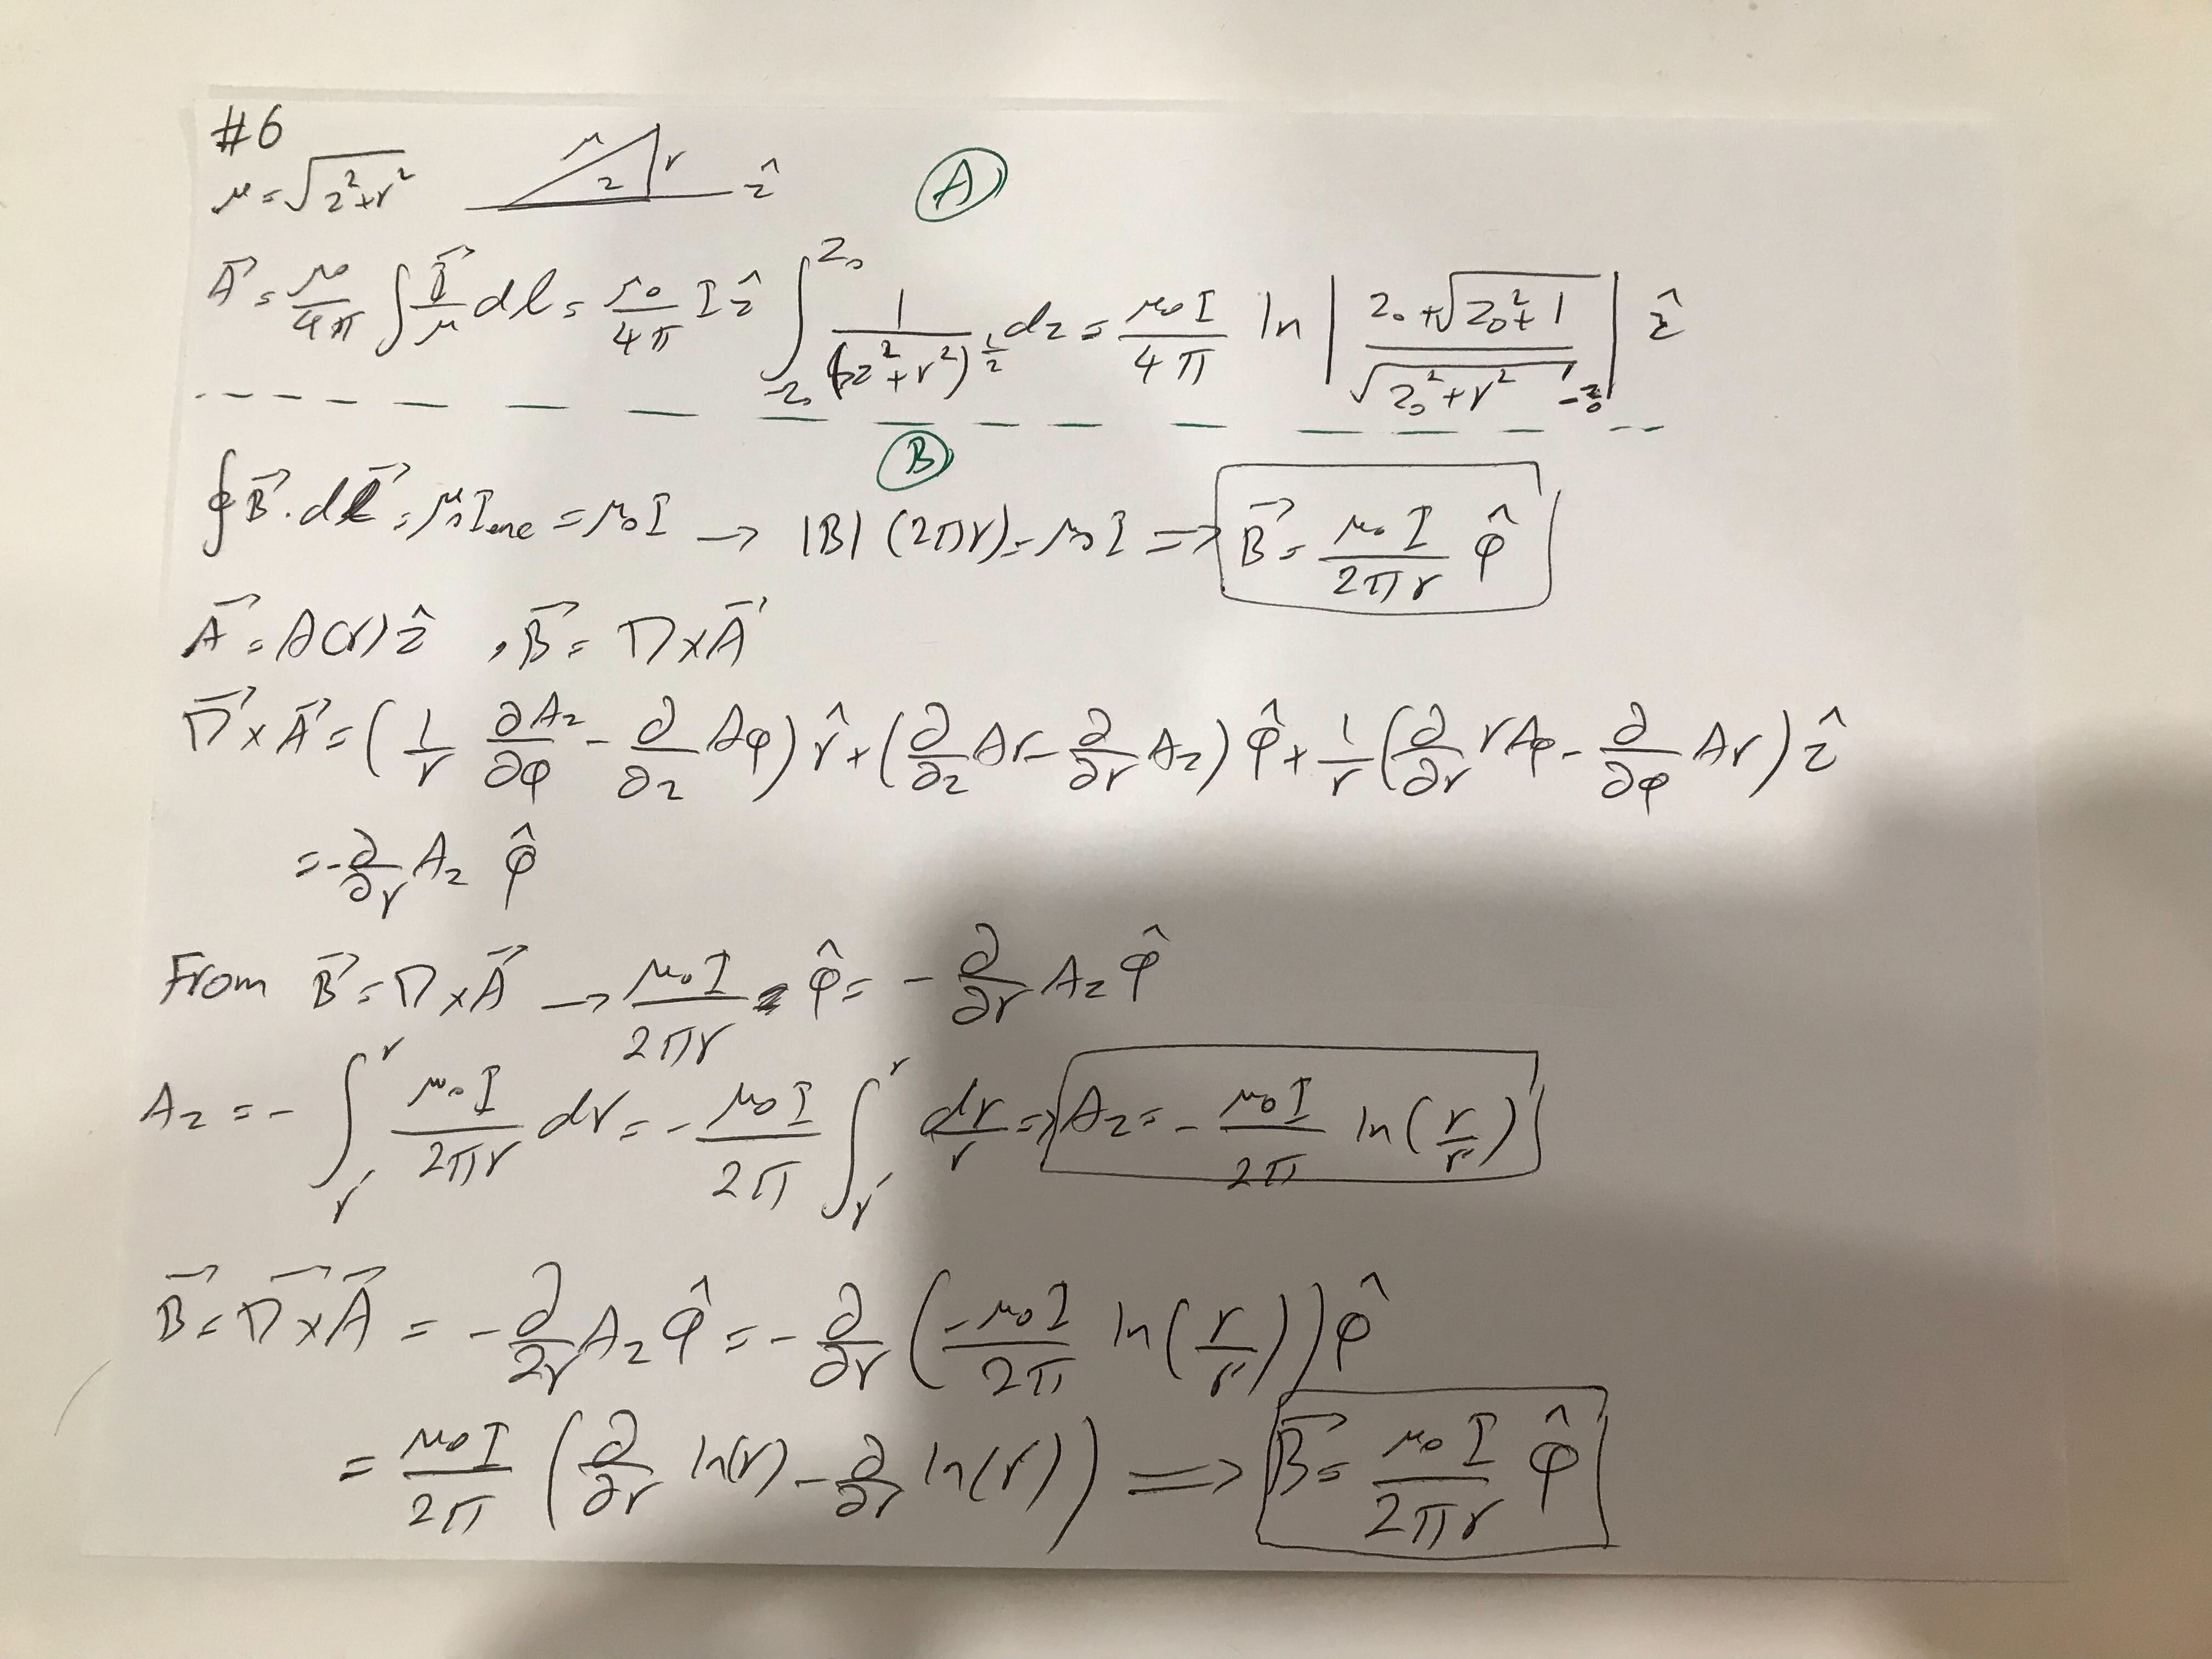
\includegraphics[height=16cm, width=17cm]{3.jpg}

      \pagebreak

      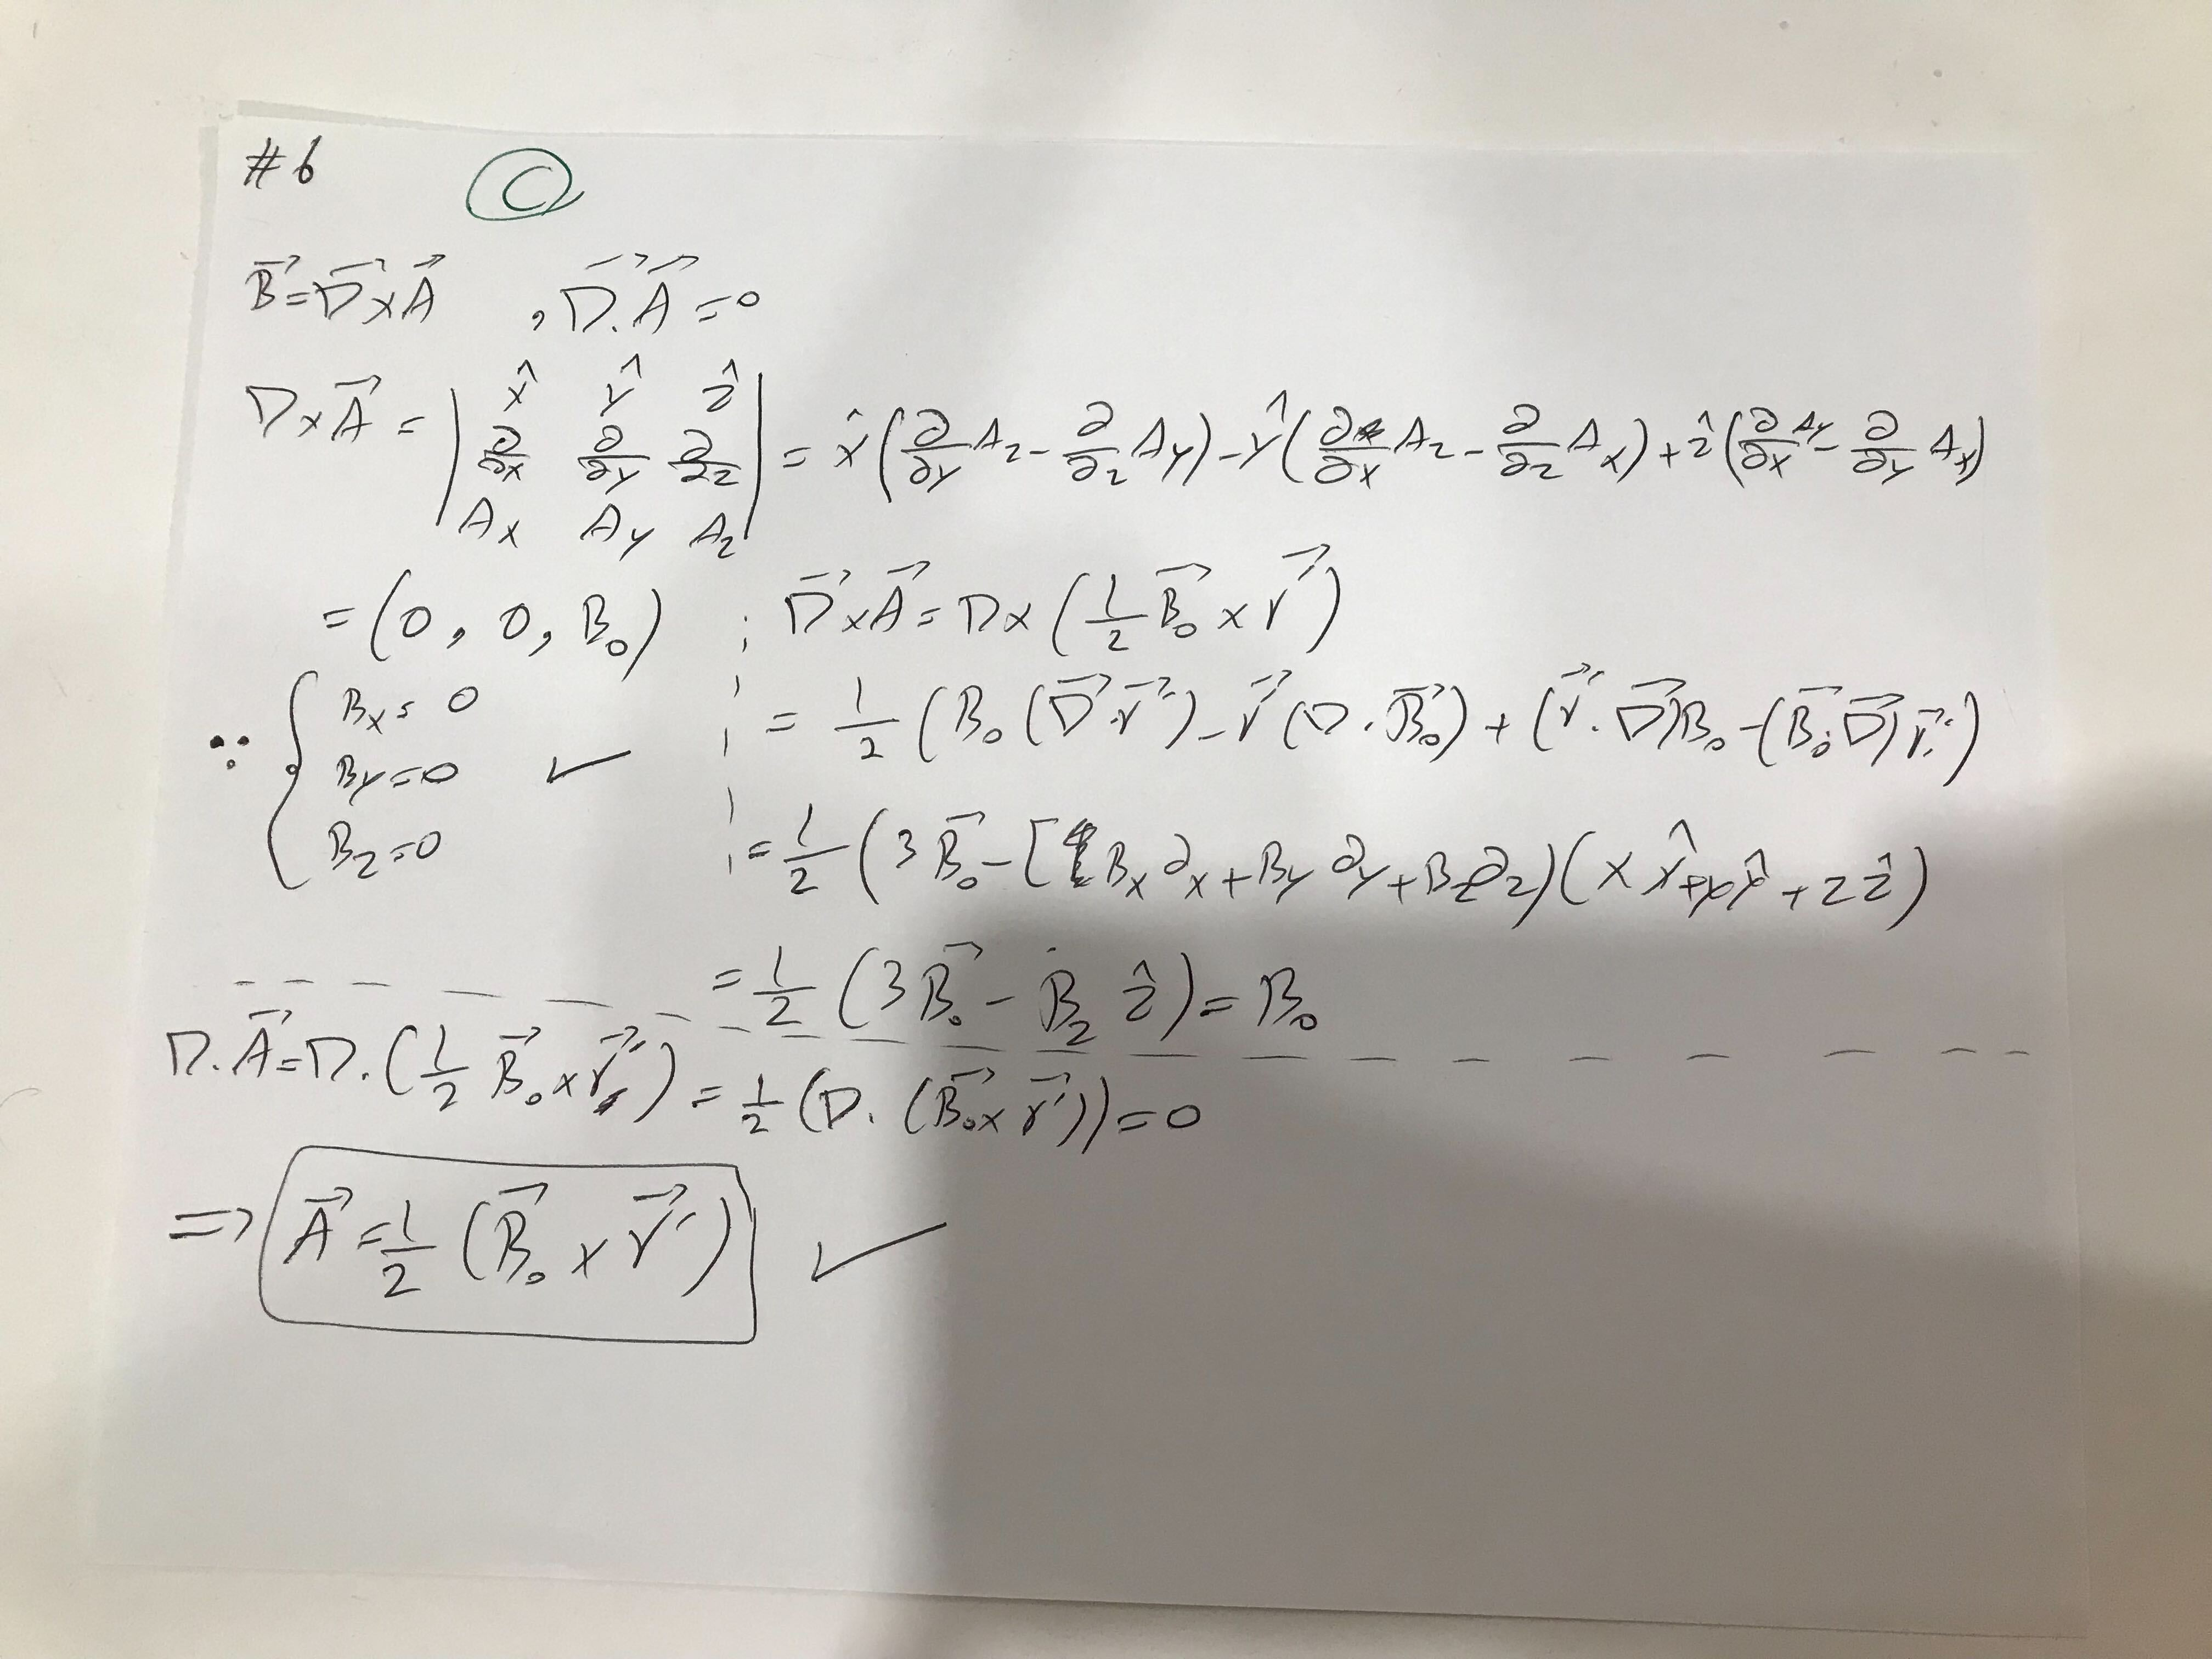
\includegraphics[height=16cm, width=17cm]{4.jpg}


  \end{enumerate}

\end{document}
